%TC:envir minttcb [ignore] xall

\chapter{Extending VTOL-AirSim: First Steps}\label{chp:extending}

This chapter is structured as a guide to developing eVTOL simulations with VTOL-AirSim and Unreal Engine 4 (UE4). The focus will be on extending the capabilities of VTOL-AirSim and understanding more of the VTOL-AirSim framework.


\section{Introduction}
Extending AirSim --- in other words, modifying or adding anything to AirSim --- involves conducting an orchestra of many diverse tools and components that all must play together in harmony to be successful. There are a number of basic components which are required in all cases, and a few components that may or may not be required depending on the needs of the project.

At some point, you will need to use \textit{Unreal Engine} --- more specifically, the \textit{Unreal Editor} --- for testing your work. In addition, you will need to integrate your work with the existing framework of VTOL-AirSim. Your project needs may also require extending the source code. Editing the source code requires a text editor: while you may use any text editor you like, we recommend Microsoft's \textit{VS Code}, for which we provide instructions for setup and use. If your project requires customizing the graphical representation of a vehicle or the environment, then you may also need to use a specialized tool for manipulating 3D computer graphics, for which we recommend the free software \textit{Blender}.

The setup process for this orchestra of tools is significantly more involved than the basic setup explained in Section~\ref{sec:basic_setup}. In this chapter, we assume that you have read Chapter~\ref{chp:userguide} (or that you understand the concepts from the chapter), and have completed the basic setup in Section~\ref{sec:basic_setup}. We begin with instructions for setting up the two core pieces for development: Unreal Engine (Section~\ref{sec:unreal_setup}) and VTOL-AirSim (Section~\ref{sec:vtolairsim_setup}).

\section{Unreal Engine Setup}\label{sec:unreal_setup}
Unreal Engine is a game engine developed by Epic Games, Inc. Its source code is written in \CC and is an open-source project on GitHub. It is known for its high-end graphics capabilities, and while it is typically used to produce video games, it has recently found use in other industries such as film, architecture, and engineering.

For our purposes, it has several advantages over a number of other game creation tools, namely that it is free for non-commercial use, has Linux support, is written in \CC and is open-source, and it has an online marketplace with a wide selection of content available to download. It also comes with a few disadvantages, including hefty system requirements, such as a moderately powerful CPU plus dedicated GPU, at least 8 GB of RAM, and at least 100 GB of available disk space on Linux. It can take well over two hours to build Unreal Engine and the Editor from source (it is required to do so on Linux) and a large amount of time to package an Unreal Editor project into a standalone application. Opening the \CC code of an Unreal Editor project with an IDE or a text editor with code analysis can be very demanding on your system due to the immense size of the code base. Furthermore, the learning curve to use the Unreal Editor is steep, and grasping the \CC API is an equally massive undertaking.

That being said, the most important reason we are using Unreal Engine is that it is the central graphics engine used by AirSim, and it was also chosen by the BYU Perception, Control and Cognition Lab for the Holodeck simulator, which we have experience with. AirSim has recently added support for the Unity game engine; however, at the time of this writing, support for it is still experimental.

\subsection{Requirements}\label{sec:unreal_requirements}
To build Unreal Engine from source, two things are required: at least 100 GB of available disk space to clone and build the engine, and your GitHub account must be a member of the \verb|EpicGames| GitHub organization. We will explain here how to meet the latter requirement.

Unreal Engine is open-source and its source code is contained in the GitHub repository \url{https://github.com/EpicGames/UnrealEngine}. However, the repository is private, and to gain access to it you must become a member of the \verb|EpicGames| GitHub organization. The instructions for becoming a member are as follows:

\begin{enumerate}
    \item Create a GitHub account if you don't already have one.
    \item Set up SSH access to GitHub (for instructions, see Appendix~\ref{apdx:github_config})
    \item Create an Epic Games account at \url{unrealengine.com}.
    \item Follow the instructions listed at \url{https://unrealengine.com/en-US/ue4-on-github} for linking your GitHub and Epic Games accounts.
    \begin{itemize}
        \item When asked, accept the End User License Agreement for \textbf{Creators}.
    \end{itemize}
    \item Join the \verb|EpicGames| GitHub organization via the email invite. You should now have access to the Unreal Engine GitHub repository.
    \item Verify by going to \url{https://github.com/EpicGames/UnrealEngine}, and you should be able to see the repository.
\end{enumerate}

\subsection{Build the Engine and Editor}
Now clone the Unreal Engine repository into a folder of your choice and build it by running the following commands. As of this writing, Unreal Engine 4.25 is the version supported by AirSim, which corresponds to the \ci{4.25} branch of the Unreal Engine repository. \textbf{Note}: Unreal Engine is very large; cloning the repository can take between 5--30 minutes, and the build process commonly takes about two hours.
\begin{minttcb}[title={Clone and Build Unreal Engine}]{bash}
    git clone -b4.25 git@github.com:EpicGames/UnrealEngine.git
    cd UnrealEngine
    ./Setup.sh
    ./GenerateProjectFiles.sh
    make
\end{minttcb}
If the build process finishes without any errors, then the engine and the Unreal Editor have successfully been built and are ready to be used. After building, the executable for the editor can be found within the repository at \ci{Engine/Binaries/Linux/UE4Editor}. To start the editor, simply execute that file in a terminal.

\section{VTOL-AirSim Setup}\label{sec:vtolairsim_setup}
The VTOL-AirSim project is a composite project that is structured, at the highest level, as an Unreal Engine \textit{Plugin}: a self-contained collection of code, asset files, and data that can be added to (or removed from) any Unreal Engine project. It is accessible as a GitHub repository at \url{https://github.com/byu-magicc/vtol-AirSim}. The VTOL-AirSim repository began as a copy of the AirSim Unreal Engine Plugin, found inside the official AirSim repository in the folder \ci{Unreal/Plugins/AirSim}, plus the AirLib code, found in the top-level folder \ci{AirLib}. From that starting point, many additions were made, along with a handful of modifications to the original code. Our work eventually resulted in the creation of a fully functional new vehicle type in AirSim for eVTOL aircraft.

Two components of the VTOL-AirSim project exist outside of the VTOL-AirSim repository: a number of large Unreal Engine asset files stored on the MAGICC Lab's Box account, and a fork of the AirSim repository found at \url{https://github.com/byu-magicc/AirSim}. To learn more about the MAGICC Lab's fork of AirSim, see \ci{MAINTENANCE.md} in the VTOL-AirSim repository.

In this text, we normally use the term \textit{VTOL-AirSim} to refer to the entire VTOL-AirSim project, as opposed to the repository itself. In the latter case, we refer to it as the \textit{VTOL-AirSim repository} if greater clarity is needed.

The full setup instructions can be found in the \ci{README.md} document of the VTOL-AirSim repository, which you can view by going to the repository's main webpage. The instructions stated there are rather detailed, so we will not repeat them in this text. Upon completing this setup, you will have the Unreal Editor running on your machine with the Blocks example project opened. The next section will detail what you need to know for working with VTOL-AirSim in the Unreal Editor.

\section{VTOL-AirSim in Unreal Editor}\label{sec:vtolairsim_unreal}

This section will serve as a concise guide on the most important concepts for using the Unreal Editor with VTOL-AirSim. The Unreal Editor is a very sophisticated software tool which is much too broad to be covered in any amount of detail in this text. Therefore, we will only cover that which is required for you to be able to do basic work with VTOL-AirSim in Unreal Editor.%
\footnote{For more information on using Unreal Editor, see the UE4 documentation at \url{https://docs.unrealengine.com}. There are also many free resources online such as web articles and YouTube videos that cover these topics.} %
In this section, we will briefly explain the key parts of the editor interface, how to run simulations in the editor, and how to package projects into standalone applications. More advanced use of the editor for customization of aircraft and environments are covered in Chapters~\ref{chp:custom_aircraft} and~\ref{chp:custom_envs}, respectively.

\subsection{Intro to Unreal Editor}
The Unreal Editor is the main graphical user interface (GUI) tool for developing video games (or engineering simulations) that use Unreal Engine. For our goals of simulating eVTOL aircraft in photorealistic environments, there are two main purposes for which the Unreal Editor is required: to \textit{modify} the graphical aspects of the simulation, and to \textit{test} modifications --- both modifications to the graphics as well as to the underlying \CC code. This means that if your project requires any customization beyond what is offered by VTOL-AirSim, then you will need to use Unreal Editor to accomplish that.

By now, you should have built and ran the Unreal Editor on your machine. When you first open the Blocks project in the editor, you will need to wait for some shaders of the Blocks environment to be compiled. Once that has finished, you will see a screen like that shown in Fig.~\ref{fig:ueditor_first_view}. Note that the interface is divided into six different \textit{panels}. In the top-left corner of each panel is a tab element which contains the name of that panel.

What follows is a quick description of each of these panels. But first, know that in UE4, a \textit{level} is the scene (or the environment, in AirSim terms) which contains every object that you see or interact with. A game is often made up of various levels; however, in our AirSim simulations, we will only have one level. When dealing with Unreal Editor, we will use the proper UE4 term of \textit{level} rather than \textit{environment}.

\begin{figure}[t]
    \centering
    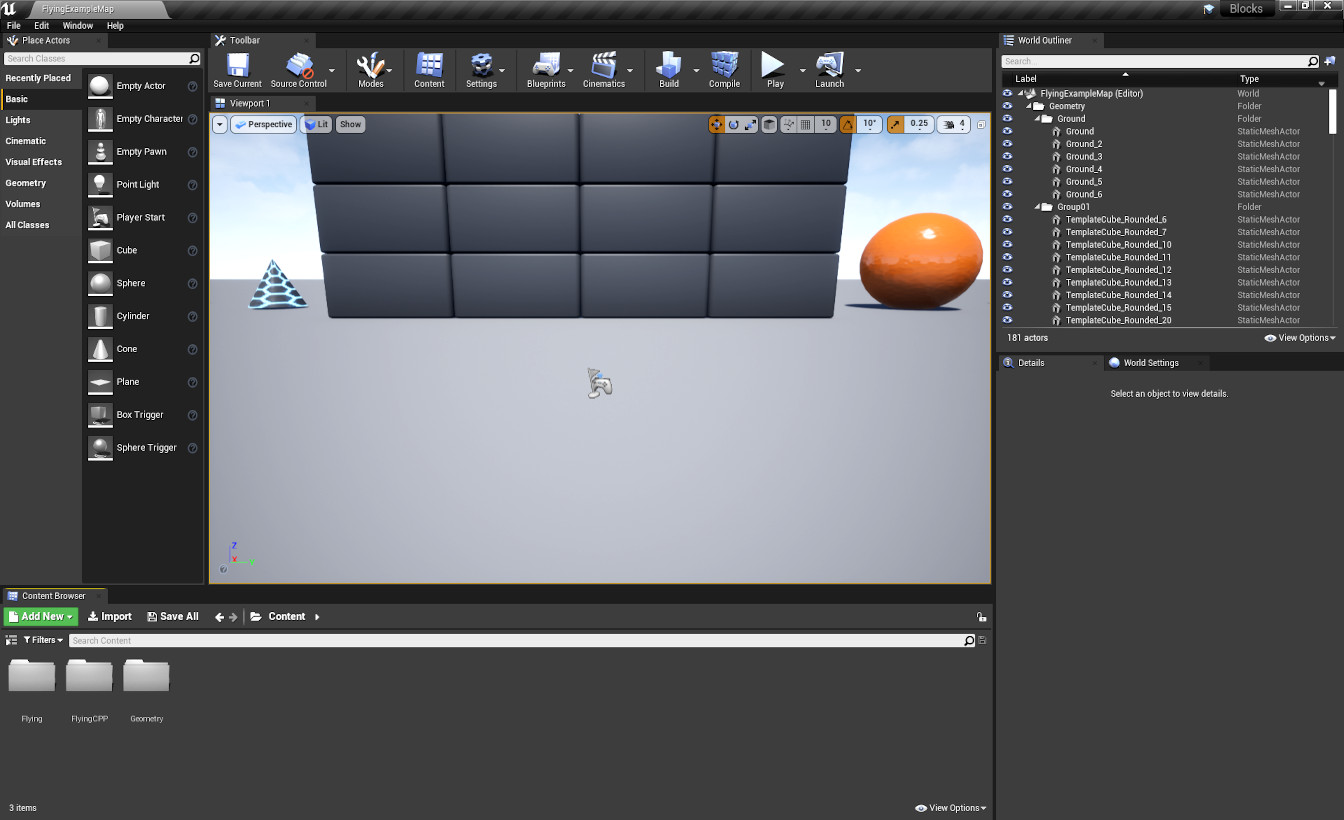
\includegraphics[width=\textwidth]{figures/ueditor_first_view}
    \caption[Unreal Editor first view]{
        The Unreal Editor with the Blocks project opened.}%
    \label{fig:ueditor_first_view}
\end{figure}

\begin{itemize}
    \item \textbf{Level Viewport} --- The center and largest panel. Here you can see and navigate around the level that the vehicle will interact with during the simulation. Because the simulation is not running, there are no vehicles visible yet. A vehicle will only spawn in the world once a simulation has started. When you press the \textbf{Play} button to begin a simulation, the \textbf{Level Viewport} will display the simulation just as it would appear in the window of a compiled environment.
    \item \textbf{Toolbar} --- Directly above the \textbf{Level Viewport}, this is where you will find the \textbf{Play} button that allows you to run a full simulation for testing (also referred to as \textit{Play In Editor} or \textit{PIE}). The other tool buttons may be ignored.
    \item \textbf{World Outliner} --- located in the upper-right of the window. This panel lists all of the \textit{Actors} that are in the scene. Actors in UE4 are any object that can be placed into a level, such as cameras, light sources, or static meshes. Currently, it only contains the Actors that are always present, but once you enter Play mode, it will additionally show dynamically spawned Actors such as one or more vehicles and the Camera Actors associated with them. Outside of Play mode, the most important Actor to be aware of is the \textbf{PlayerStart} Actor: its \textit{Location} and \textit{Rotation} (the terms in UE4 used for position and orientation, respectively) in the level are used by AirSim as the position and orientation for its internally-computed global coordinate frame. This means you can move \textbf{PlayerStart} to change where vehicles spawn in AirSim as well as what is set as the global (0, 0, 0) position and orientation.
    \item \textbf{Details} --- located in the lower-right of the window. When you click on an Actor in either the \textbf{Level Viewport} or the \textbf{World Outliner}, its configurable attributes will be found here. The key item to note in this panel is that here you can modify the \textit{Transform} of an Actor, which includes its Location, Rotation, and Scale attributes.
    \item \textbf{Place Actors} --- located at the left of the window. This panel contains a number of Actors provided by UE4 which you may place in the level.
    \item \textbf{Content Browser} --- located at the bottom of the window. Here you will find all the \textit{Assets} (or \textit{content}) that are part of the currently opened Unreal Project. The terms \textit{Assets} and \textit{content} as well as the Content Browser are covered in the next section, Section~\ref{sec:content_vtolairsim}.
\end{itemize}

\subsection{Content of VTOL-AirSim}\label{sec:content_vtolairsim}
This section will cover the UE4 content that is part of VTOL-AirSim. In UE4, the term \textit{content} refers to the objects or functionalities that make up a game (i.e., simulation) that is not \CC code. Examples of content types include Textures, Materials, Static Meshes, or Blueprints. An \textit{Asset} is a binary file that stores content. The \textbf{Content Browser} is like a special file manager that shows you all the assets that are part of the project.

By default, the editor will have open the \ci{Content} folder of the project. In our case, this is the folder \ci{Blocks/Content}. To more easily view the directory structure, click on the small icon to the left of \textbf{Filters} to reveal the \textbf{Sources panel}. You will find that the files and folders located in \ci{Blocks/Content} and in the Content Browser mostly match, with some files and folders hidden from view. The assets that we are actually interested in are not in \ci{Blocks/Content}, however, but rather in \ci{Blocks/Plugins/vtol-AirSim/Content}. To instead view these files, click on \textbf{View Options} at the bottom-right of the \textbf{Content Browser}, and check the box for \textbf{Show Plugin Content}. The \textbf{Sources panel} should now show a new folder named \ci{AirSim Content}. This folder is so named because the VTOL-AirSim Plugin actually retains its original title of \texttt{AirSim} within Unreal Engine; but it is in fact the folder \ci{Blocks/Plugins/vtol-AirSim/Content}. See Appendix~\ref{apdx:unreal_paths} for more information on path names in UE4.

There are 3 directories inside \ci{AirSim Content} that we wish to highlight:
\begin{enumerate}
    \item \ci{Blueprints} --- Here you will find the \textit{Blueprints} of several very important Actors in AirSim; in particular, the Actor for the multirotor vehicle, \ci{BP_FlyingPawn}.
    \item \ci{Models/QuadRotor1} --- This folder contains the Static Meshes, Materials, and Textures that compose the multirotor vehicle, which are specified in \ci{BP_FlyingPawn}.
    \item \ci{VTOL} --- All assets that are unique to VTOL-AirSim are contained here. Currently there is only one subdirectory, \ci{Tiltrotor}, however any custom eVTOL aircraft that may be added will go here. Inside the \ci{Tiltrotor} folder is all of the assets that make up the tiltrotor vehicle, including the equivalent \ci{BP_TiltrotorPawn} Blueprint and the Static Meshes and Materials that it is composed of, similar to the multirotor vehicle.
\end{enumerate}

Another asset, the \ci{AirSimAssets} Level, is important specifically for packaging a project, as is explained in Section~\ref{sec:packaging}.

\subsection{Play In Editor}
The most useful feature of the editor for our purposes is \textbf{Play In Editor} (\textbf{PIE}), accessed via the \textbf{Play} button. This is how you will test changes you've made to VTOL-AirSim, whether they are graphical changes made in the editor, or changes made to the source code (though changes to the code will require closing the editor and rebuilding the project before they will be active). Play In Editor allows you to preview a VTOL-AirSim simulation just as you would see in a standalone application, but displayed within the \textbf{Level Viewport}. It also has a few extra features, such as \textbf{Pause} to pause the simulation, and \textbf{Eject} to become a third-person observer where you can click on objects in the scene, such as the aircraft in the simulation, and see real-time attributes about it in the \textbf{Details} panel. For example, you could select the tiltrotor vehicle's engines to see their exact angle values while the simulation is running, and see the values change in real time. Keep in mind that you won't have the same performance using Play In Editor that you will when running a standalone application, but you should still have decent performance.

\subsection{Package a Project}\label{sec:packaging}
When you are satisfied with the changes you've made to VTOL-AirSim or your Unreal Project, you can package your project into a standalone application. This is how the compiled environments from AirSim and VTOL-AirSim are made. This allows you to get more performance out of your simulation as well as share your simulation environment with others.

There is an interesting quirk about the AirSim Plugin in Unreal Engine that is very important to know if you are going to package your project. Notice how in the \textbf{World Outliner} panel there are no tiltrotor, multirotor, or car vehicles in the scene. This is because in AirSim the vehicles that are part of the simulation are spawned at runtime; they are not permanent objects in a level. However, in Unreal Engine, only the Actors which appear in at least one level are packaged into a game. Therefore, the tiltrotor, multirotor, and car vehicles of AirSim must be present in at least one level at the time of packaging. If you specify a simulation mode in your settings file but that specific vehicle was not a part of any level, then the application will crash with an error that says \ci{Couldn't find file for package} proceeded by the path to the vehicle's Blueprint, as specified in the source code.

AirSim's solution to this is the \ci{AirSimAssets} Level, found under \ci{AirSim Content}. Double-click this level to open it, and you will see in the \textbf{World Outliner} these three vehicles, plus the Actor for \ci{ComputerVision} mode. The \textbf{Level Viewport}, however, will be completely empty and black; this is because the level contains no lighting, as it doesn't need any. It is simply a dummy level to work with Unreal Engine's packaging system.

In order to package the tiltrotor vehicle into compiled environments, we had to add the tiltrotor's Blueprint, \ci{BP_TiltrotorPawn}, to this level. If you create a custom aircraft, you will also need to add it to this level. You can click and drag the Blueprint of your custom vehicle anywhere onto the \textbf{Level Viewport} when this level is loaded (the location does not matter), and that is enough to comply with this UE4 requirement. Go back to the default Blocks level by navigating to \ci{Content/FlyingCPP/Maps} and double-clicking on \ci{FlyingExampleMap}.

Packaging a project is a simple, yet lengthy process. All you need to do is go to \textbf{File > Package Project > Linux > Linux}, choose a suitable directory to store your packaged environment, and then click \textbf{Open} and it will begin the process of packaging the project. The process can take over 30 minutes, even for the simple Blocks project on moderate computer hardware, so be prepared for that. Packaging is quicker if you choose the same directory the next time you package the project as it will only do an iterative build rather than build the complete project.

When the packaging process has completed, navigate inside the \ci{LinuxNoEditor} directory that was created, and run the \ci{.sh} file for your project just as you would with any compiled AirSim environment.

\section{Development Using VS Code}
VS Code is the text editor that we recommend for editing the VTOL-AirSim source code. Due to the massive size of the UE4 \CC libraries, it can be very demanding on your machine to edit using the code analysis features of VS Code; however, the cost is usually outweighed by the many benefits it brings for navigating and analyzing the \CC code.

The first thing you should do is install the C/\CC extension for VS Code. Next, rather than open specific \textit{files} to edit, you should open \textit{directories} for editing. The easiest way to do this is to run in a terminal \ci{code <path>}, where \ci{<path>} is the path to the directory you want to open for editing files in VS Code. For working with the VTOL-AirSim code, you can open your Unreal Engine Project that contains the VTOL-AirSim Plugin and that you will use for testing, or you can open the \ci{Plugins/vtol-AirSim} directory, or lastly you can open just the \ci{Source/AirLib} directory of VTOL-AirSim if you won't need to see any of the Unreal Engine code.

You need a special \ci{c_cpp_properties.json} file present that tells VS Code what directories to include when searching for \CC header or source files. Without this file, the C/\CC extension won't be able to do code analysis for any files that are outside the directory of the file currently being edited. There is a vast number of directories that make up the UE4 libraries, so you shouldn't create this file yourself. There is a script in the Unreal Engine repository that will do this for you named \ci{GenerateProjectFiles.sh}. The script is invoked with the syntax:
\begin{minttcb}[title={}]{bash}
GenerateProjectFiles.sh <path to Blocks>/Blocks.uproject -game -engine
\end{minttcb}
If you are using a project other than Blocks, replace \ci{Blocks} with the name of your project. This will create a number of files into your project's top-level directory for several different IDEs and text editors, but the files for VS Code are placed in a hidden directory named \ci{.vscode}. One of those files is \ci{c_cpp_properties.json}. It contains a great number of include directories to allow the C/\CC extension to do its job correctly. If you open your Unreal Project directory in VS Code, then you should be ready to start editing the code. However, since you won't need to edit any of the files outside of the VTOL-AirSim plugin, you can also copy the \ci{.vscode} directory to the \ci{Plugins/vtol-AirSim} directory, and then open just the \ci{vtol-AirSim} directory to reduce the number of files for VS Code to search through.

\section{Build}
You need to build all the VTOL-AirSim code in order to see your changes reflected in Unreal Editor. There is a guide document with build instructions located in the VTOL-AirSim GitHub repo at \url{https://github.com/byu-magicc/vtol-AirSim/blob/main/DEVELOPMENT.md}. The guide will teach you all you need to know about building the code.

Once you have completed all these setup steps, you are ready to begin developing and customizing VTOL-AirSim. In the next chapters, we show how you can create custom aircraft and environments for your own simulations.